\documentclass[10pt,twocolumn,letterpaper]{article}

% Pacotes basicos - maxima compatibilidade Windows
\usepackage{geometry}
\usepackage{times}
\usepackage{titlesec}
\usepackage{url}
\usepackage{graphicx,xcolor,comment,enumerate,multirow,multicol} 
\usepackage{amsmath,amsthm,amsfonts,amssymb,dsfont,mathtools, array}
\usepackage[brazil]{babel}

\usepackage{enumitem}
\setlist[itemize]{
    itemsep=2pt,        % Espaçamento vertical entre itens
    parsep=0pt,         % Espaçamento entre parágrafos dentro de um item
    topsep=0pt,         % Espaçamento vertical antes do primeiro item da lista
    partopsep=0pt,      % Espaçamento extra quando a lista começa no início de um parágrafo
    leftmargin=1.5em    % Opcional: Ajusta a margem esquerda (se estiver muito indentado)
}

% Configuracao da pagina
\geometry{
    letterpaper,
    left=0.75in,
    right=0.75in,
    top=0.75in,
    bottom=1in
}

%% Edição confortável
% Inclui o pacote xcolor com a opção para nomes de cores
\usepackage[svgnames]{xcolor}
% Para desativar comente a linha utiliando %
%% Define a cor do texto usando o código hexadecimal
\definecolor{Cornsilk}{HTML}{FFF8DC}

% Define a cor de fundo da página como preta
\pagecolor{Black}

% Define a cor padrão do texto para todo o documento
\color{white}

% Configuracao das secoes
\titleformat{\section}[block]
{\normalfont\fontsize{10}{12}\bfseries}
{\thesection.}{0.5em}{}

% Remove numeracao das paginas
\pagestyle{empty}

% Configuracoes de espacamento
\setlength{\columnsep}{0.25in}
\setlength{\parindent}{0pt}
\setlength{\parskip}{6pt}

\begin{document}

% Titulo centralizado em coluna unica
\twocolumn[
\begin{center}
    {\fontsize{16}{19}\selectfont\bfseries 
    Experimento 4 - Diodo semicondutor}

    \vspace{1cm}
    
    {\fontsize{11}{13}\selectfont 
     Carlos Eduardo da S. Papa – 232013390, Ronan Cunha Freitas – 232013425 }

    \vspace{0.25cm}   

    {\fontsize{11}{13}\selectfont 
    Turma 02}
    
    \vspace{.25cm} 
\end{center}
]

\section{OBJETIVOS}

\hspace{1cm} Levantar a curva característica $I_D\times V_D$ para o diodo BY127 e analisar a curva de resposta para os modelos de circuito com esse diodo.

\vspace{.25cm}

\section{MATERIAIS e EQUIPAMENTO UTILIZADOS}

\begin{itemize}
    \item 2 diodos BY127;
    \item Fonte de tensão;
    \item Gerador de função;
    \item Osciloscópio;
    \item 2 multímetros;
    \item Resistor de $1\,k\Omega$;
    \item Capacitor de $10\,\mu F$
    \item Cabos para conexão e protoboard;
\end{itemize}

\vspace{.25cm}

\section{PROCEDIMENTOS EXPERIMENTAIS}

\noindent\textit{A. Curva característica do diodo BY127.}

\hspace{1cm}Após a montagem do circuito devemos variar a queda de tensão do diodo VD em passos de 100 mV e anotar a corrente ID que passa pelo circuito. A corrente não pode passar de 40 mA para que o diodo não queime. 

\hspace{1cm}Para finalizar esta etapa, devemos inventer os terminais da fonte e repetir o mesmo procedimento com o diodo reversamente polarizado.

% \vspace{-.25cm}

\begin{figure}[h]
    \centering
    \includegraphics[width=5cm]{imagens/figA.pdf}
    \caption{Circuito do procedimento A}
    \label{fig:CircA}
\end{figure}

\noindent\textit{B. Análise de Circuitos com diodos BY127.}

\hspace{1cm}Nesta etapa devemos montar cada circuito apresentado na figura 2. A fonte em cada circuito é um sinal senoidal com amplitude 8 Vpp e frequencia de 100 Hz.

\hspace{1cm}Para cada circuito devemos fotografar e relatar a curva de entrada e a curva de saída observada osciloscópio, lembrando sempre de destacar a atenuação e defasagem entre as curvas.

\vspace{-.5cm}

\begin{figure}[h]
    \centering
    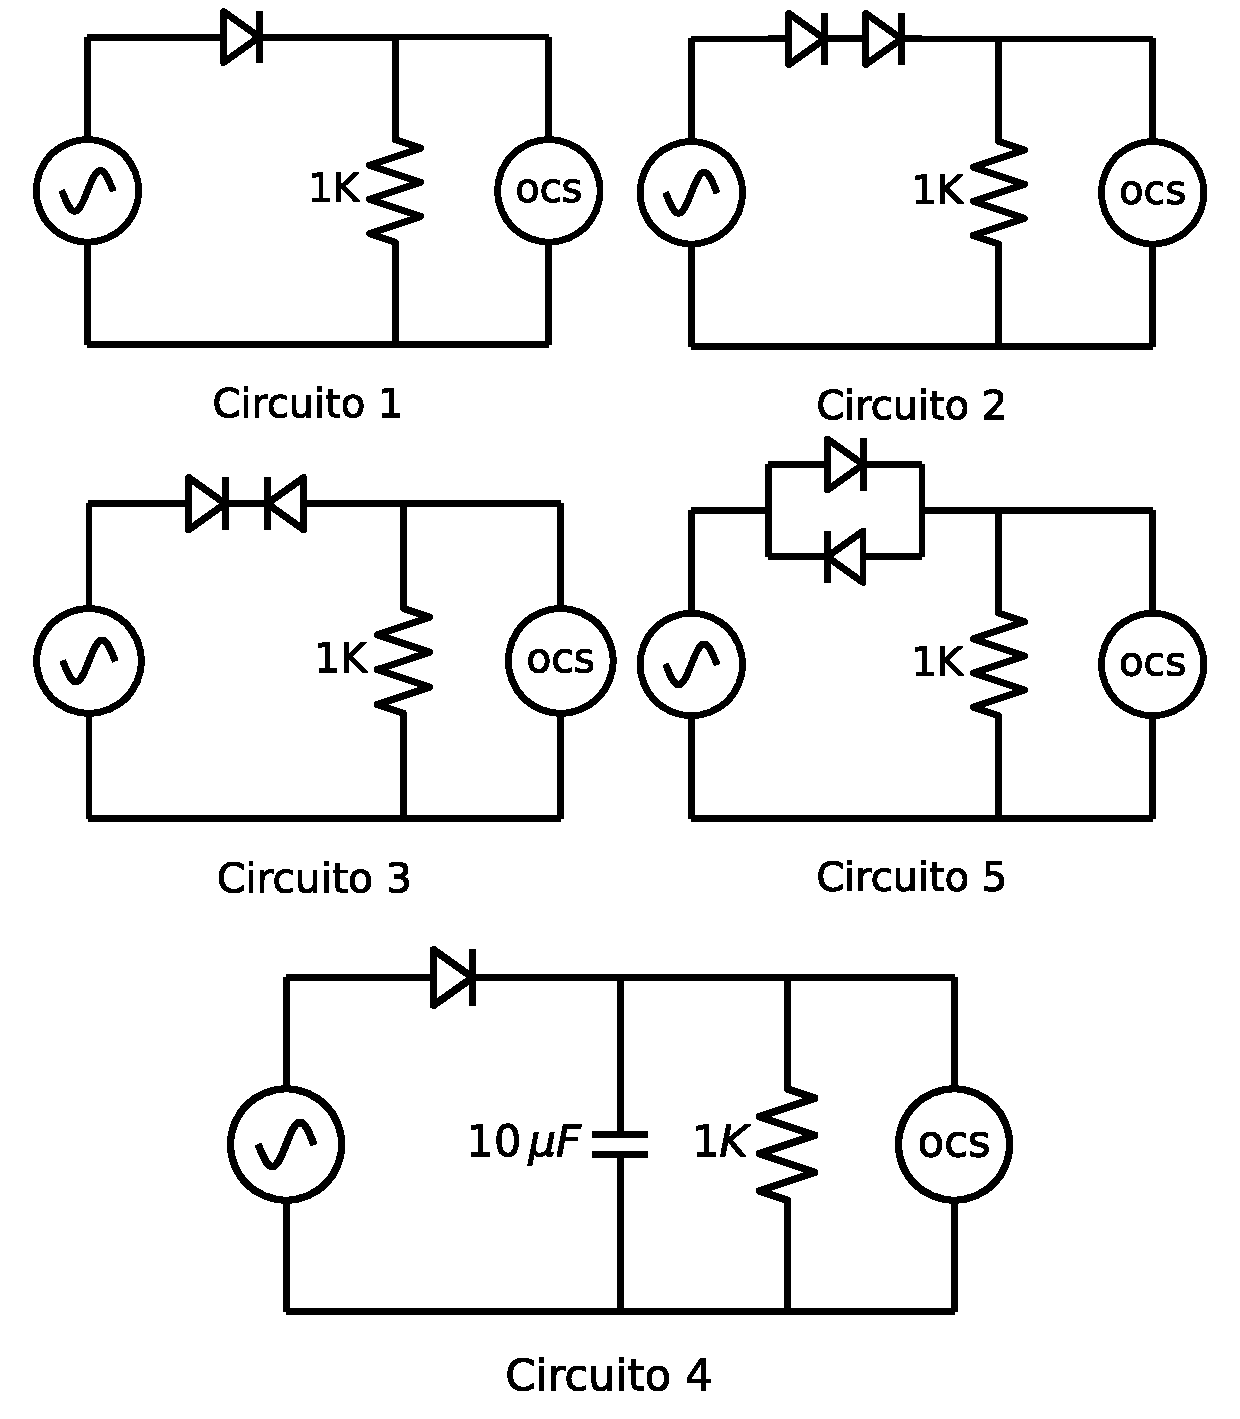
\includegraphics[width=7cm]{imagens/FigB.pdf}
    \caption{Circuitos do procedimento B}
    \label{fig:CircB}
\end{figure}

\vspace{-.75cm}

\section{RESULTADOS EXPERIMENTAIS}

\noindent\textit{A. Curva característica $I_D\times V_D$.}

\hspace{1cm} Ao realizar a parte A do procedimento obtivemos os dados necessários para levantar a curva característica do diodo. Os dados estão relatados na tabela I e a curva característica pode ser vista na figura 3.

% \vspace{-.25cm}

\begin{table}[!h]
    \centering
    \caption{Medidas Obtidas para Obter a Curva}
    \label{tab:medidas}
    \vspace{0.25cm}
    \begin{tabular}{ccc}
        \hline
        \rule{0pt}{3ex} $ V_D \,\,[V]$ & & $ I_D \,\, [mA]$ \\[5pt]
        \hline
        \rule{0pt}{3ex}-0.8 & & 0 \\
        -0.7 & & 0 \\
        -0.6 & & 0 \\
        -0.5 & & 0 \\
        -0.4 & & 0 \\
        -0.3 & & 0 \\
        -0.2 & & 0 \\
        -0.1 & & 0 \\
        0 & & 0 \\
        0.1 & & 0 \\
        0.2 & & 0 \\
        0.3 & & 0 \\
        0.4 & & 0 \\
        0.5 & & 0.7 \\
        0.6 & & 3.3 \\
        0.7 & & 29.7 \\
        0.77 & & 30.4 \\[5pt]
        \hline
    \end{tabular}
\end{table}

\vspace{-.25cm}

\begin{figure}[h]
    \centering
    \includegraphics[width=8cm]{imagens/grafico_ID_x_VD.png}
    \caption{Curva característica $V_D\times I_D$}
    \label{fig:VD_ID}
\end{figure}

\noindent\textit{B. Análise de Circuitos com diodos BY127.}

\hspace{1cm} Ao realizar a parte B do procedimento obtivemos as curvas de tensão entrada e de saída para cada circuito, anotando a atenuação e defasagem de cada um na tabela II.

% \vspace{-.25cm}

\begin{figure}[!h]
    \centering
    \includegraphics[width=7cm]{fotos/1.jpg}
    \caption{Circuito 1}
    \label{fig:circ1}
\end{figure}

% \vspace{-.25cm}

\begin{figure}[!h]
    \centering
    \includegraphics[width=7cm]{fotos/1.jpg}
    \caption{Circuito 2}
    \label{fig:circ2}
\end{figure}

% \vspace{-.25cm}

\begin{figure}[!h]
    \centering
    \includegraphics[width=7cm]{fotos/1.jpg}
    \caption{Circuito 3}
    \label{fig:circ3}
\end{figure}

% \vspace{-.25cm}

\begin{figure}[!h]
    \centering
    \includegraphics[width=7cm]{fotos/1.jpg}
    \caption{Circuito 4}
    \label{fig:circ4}
\end{figure}

% \vspace{-.25cm}

\begin{figure}[!h]
    \centering
    \includegraphics[width=7cm]{fotos/1.jpg}
    \caption{Circuito 5}
    \label{fig:circ5}
\end{figure}

% \vspace{-.25cm}

\begin{table}[!h]
    \centering
    \caption{Defasagem e Atenuação dos Circuitos}
    \label{tab:defasagem}
    \vspace{0.25cm}
    \begin{tabular}{ccc}
        \hline
        \rule{0pt}{3ex}\textbf{Circuito} & \textbf{Defasagem} [ms] & \textbf{Atenuação} [V]\\[5pt]
        \hline
        \rule{0pt}{3ex} 1 &  & \\
        2 &  & \\
        3 & - & - \\
        4 &  & \\
        5 &  & \\[5pt]
        \hline
    \end{tabular}
\end{table}

\section{ANALISE DOS RESULTADOS EXPERIMENTAIS}

\noindent\textit{A. Curva característica do diodo BY127.}

\hspace{1cm}A análise dos valores apresentados na Tabela I e da curva mostrada na Figura 3 evidencia o comportamento típico do diodo BY127 sob diferentes condições de polarização. 

\hspace{1cm}Observa-se que, quando submetido à polarização direta, o dispositivo inicia a condução de corrente de forma significativa apenas para tensões superiores a aproximadamente $0.6 \, V$. Por outro lado, para valores de $V_D$ inferiores a zero, correspondentes à polarização reversa, não foi registrada condução apreciável, mantendo-se a corrente praticamente nula.

\hspace{1cm}Esse comportamento está em consonância com as especificações presentes no datasheet do BY127, que indicam tensão de limiar entre $0.6 \, V$ e $0.8 \, V$ e corrente desprezível na região de polarização reversa. Assim, os resultados obtidos confirmam o regime de operação esperado para esse tipo de diodo retificador.

\noindent\textit{B. Análise de Circuitos com diodos BY127.}

\hspace{1cm}Os resultados referentes à segunda parte do experimento, sintetizados na Tabela II, permitem observar que o diodo real pode ser interpretado como um diodo ideal acrescido de uma queda de tensão em série. Essa característica manifesta-se diretamente na atenuação verificada entre as tensões de entrada e saída, evidenciando o comportamento não ideal do componente.

\hspace{1cm}A Figura 4 ilustra o funcionamento típico de um retificador de meia onda: a condução ocorre apenas durante a semiciclo positivo, enquanto a polarização reversa do diodo bloqueia a passagem de corrente no semiciclo negativo. Já a Figura 5 apresenta maior atenuação relativa, resultado da utilização de dois diodos em série, cada um contribuindo com sua respectiva queda de tensão.

\hspace{1cm}Na configuração ilustrada na Figura 6, os diodos encontram-se polarizados de forma oposta, o que impede a condução em ambos os semiciclos e faz com que o circuito se comporte como um circuito aberto, independentemente da tensão aplicada. Em contraste, no caso mostrado na Figura 8, os diodos estão dispostos em paralelo, de modo que o caminho de condução depende da polaridade da fonte: o diodo superior conduz na polarização direta e o inferior conduz na polarização reversa.

\hspace{1cm}Por fim, o circuito correspondente à Figura 7 representa um retificador com capacitor de filtro, também conhecido como retificador de pico. Nesse arranjo, considerando $V_{in}$, $V_{out}$ e $V_t$ como as tensões de entrada, saída e queda no diodo, respectivamente, observam-se dois regimes distintos. Inicialmente, quando $V_{in} > V_{out}$, o diodo conduz e o capacitor carrega até o valor máximo da onda de entrada. Em seguida, com o diodo despolarizado, o capacitor passa a fornecer energia à carga, produzindo uma descarga exponencial dada por $V_{out} = V_{in} \, e^{-t/RC}$. Quando a tensão de entrada volta a superar a tensão no capacitor, o ciclo de carga se reinicia.

\section{Conclusão}

\hspace{1cm}Os resultados obtidos e a análise subsequente permitiram compreender de forma abrangente o comportamento do diodo BY127 tanto em regime de polarização direta quanto reversa. Evidenciou-se, ainda, a versatilidade do componente em aplicações de circuitos eletrônicos, especialmente no contexto de retificação e condicionamento de sinais. A comparação entre os dados experimentais e a teoria consolidada mostrou-se coerente, reforçando a confiabilidade do procedimento adotado e a adequação dos modelos teóricos empregados.

\section{REFERENCIAS BIBLIOGRAFICAS}

{\small
\begin{enumerate}

    \item CESCHIN, Artemis M. Apostila de materiais eletricos e magneticos.

    \item REZENDE, Sergio M. Materiais e Dispositivos Eletrônicos. 2ª ed. São Paulo: Editora Livraria da Física, 2004.

    \item VISHAY, Miniature Glass Passivated Junction Rectifier, BY127MGP datasheet, 12/03/2012.
    
\end{enumerate}
}

\end{document}